\documentclass[12pt,a4paper]{article}
 
\usepackage{float}
%für feststellen der figures und tables [H] dranschreiben
\usepackage{units}
%wird so benutzt: 
%\unit[value/Zahl]{dimension/Einheit} oder 
%\unitfrac[value/Zahl]{dimension/Einheit num/Zähler}{dimension/Einheit denum/Nenner} oder
%\nicefrac[fontcommand/Schriftart]{dimension/Einheit num/Zähler}{dimension/Einheit denum/Nenner}

\usepackage{caption}
\usepackage{subcaption}

\usepackage[left=2cm,right=2cm,top=2cm,bottom=2cm]{geometry}
\usepackage[utf8]{inputenc}
\usepackage[T1]{fontenc}
\usepackage{lmodern}
\usepackage[ngerman]{babel}
\usepackage{amsmath}
\usepackage{graphicx}
 
\title{Regelschaltungen}
\author{Frederik Strothmann, Henrik Jürgens}
\date{\today}
%niemals zwei überschriften direkt übereinander schreiben, also immer mindestens in einem satz was sinnvolles unter jede überschrift schreiben (bei den versuchen z.B. das versuchsziel) 
\begin{document}
%deckblatt erstellen.
\maketitle
\newpage
\tableofcontents
\newpage
\section{Einleitung}
%einleitung zu dem experiment.
%auf die einstellungen, die vor dem versuch gemacht werden, eingehen oder auf eine anleitung dazu verweisen
%es soll immer erwähnt werden um was es in dem Versuch geht und wie das relisiert werden soll
%---------------------------------------------------------------------------------------------
%hinter der einleitung kann der allgemeine theoretische hintergrund in einer zusätzlichen section erklärt werden
%1-----------------------------------------------1

In diesem Versuch werden Regelschaltungen untersucht, dies finden in den meisten heutzutage erhältlichen Geräten Anwendung, z.B Computer und Autos. Es werden vier verschieden Regelschaltungen untersucht, eine Zweiwegregelung, eine Zweiwegregelung mit Hysterese, eine Proportionalregelung und eine Proportionalregelung mit Integrator.


\section{Eichung des NTC-Sensors}
%kurz das ziel dieses versuchsteiles ansprechen, damit keine zwei überschriften direkt übereinander stehen!
%bei schwierigeren versuchen kann auch der theoretische hintergrund erläutert werden. (mit formeln, herleitungen und erklärungen)
Im ersten Versuchsteil soll der NTC-Sensor für die nachfolgenden Messungen geeicht werden. Der NTC-Sensor ist ein Widerstand, der Exponentiell von der Temperatur abhängt.

\subsection{Verwendete Geräte}
%(immer) eine skizze oder ein foto einfügen, die geräte/materialien !nummerieren! und z.b. eine legende dazu schreiben, besser wäre es das ganze in einem Fließtext gut zu beschreiben.
%falls am anfang des versuches nicht klar ist, was alles verwendet wird, wenn möglich erst am ende ein großes foto von den verwendeten materialien machen!\\.

Es werden ein NTC-Sensor, ein Kühlkörper, ein DMM, ein Heizwiderstand und ein Netzgerät verwendet.

\subsection{Verwendete Formeln}
%eine legende kann angefertigt werden, die selbstverständlichen buchstaben müssen nicht extra erklärt werden
%mit knappen erklärungen die !verwendeten! formeln, sowie die zugehörige fehlerrechnung einfügen
%2-----------------------------------------------2
%ab hier kann nochmal in einzelne versuchsteile unterteilt werden

Der Zusammenhang zwischen Widerstand und Temperatur ist durch Gleichung \ref{eqn:ntc} gegeben. R$_{25}$ ist der Widerstand bei 25$^\circ$C

\begin{align}
\text{R}_\text{NTC}(\text{T}) = \text{R}_{25} \text{exp}\left(-\text{B} \left(\frac{1}{\text{T}_{25}}-\frac{1}{\text{T}}\right)\right)
\label{eqn:ntc}
\end{align}

\subsection{Versuchsaufbau}
%skizze zum versuchsaufbau (oder foto) einfügen,   es muss erklärt werden wie das ganze funktioniert und welche speziellen einstellungen verwendet wurden (z.b. welche knöpfe an den geräten für die messung verdreht wurden)

1 ist der NTC, 2 ist der Kühlkörper und 3 der Heizwiderstand.

\begin{figure}[H] 
  \centering
    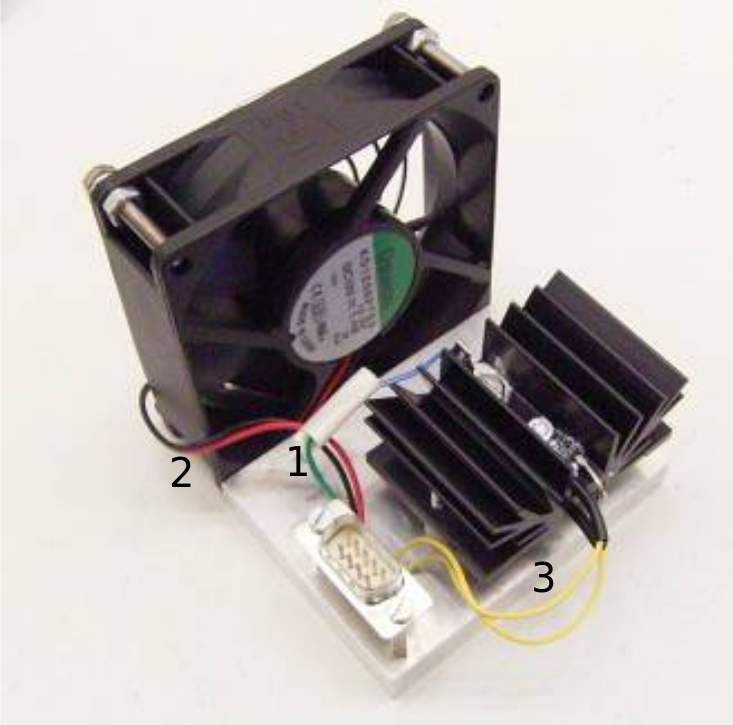
\includegraphics[ scale = 0.3]{Auf_1.png}
  	\caption[Aufbau zur Eichung des NTC]{Aufbau zur Eichung des NTC\footnotemark}
  \label{fig:auf_1}
\end{figure}
\footnotetext{Abbildungsteile entnommen von http://www.atlas.uni-wuppertal.de/$\sim$kind/ep7\_14.pdf am 06.12.2014}

\subsection{Versuchsdurchführung}
%erklären, !was! wir machen, !warum! wir das machen und mit welchem ziel
%(wichtig) präzize erklären, wie bei dem versuch vorgegangen und was gemacht wurde

Es wurde der Versuchsaufbau wie in Abbildung \ref{fig:auf_1} genommen und die grünen Kabel (der NTC) an ein DMM für die Widerstandsmessung angeschlossen. Danach wird der Heizwiderstand (das schwarze und das rote Kabel) an die 20V Gleichspannungsquelle des Netzgerätes angeschlossen. Dann wird das Digitalthermometer in die Bohrung des Hitzewiderstandes gesteckt und die Messung des Widerstandes in Abhängigkeit der Temperatur begonnen.

\subsection{Messergebnisse}
%die messwerte in !übersichtlichen! tabellen angegeben
%zu viele kleine tabellen in große tabellen überführen!
%zu große tabellen mit dem [scale]-befehl scalieren oder (falls zu lang) in zwei kleinere tabellen aufteilen
%(wichtig) vor !jeder! tabelle sagen, was gemessen wurde und wie die fehler gewählt wurden und ausreichend !erklären!, !warum! wir unsere fehler grade so gewählt haben

Der Fehler der Temperatur wurde mit dem Ablesefehler bestimmt, da kein Fehle angeben war, er beträgt 0,1$^\circ$C. Der Fehler des Widerstandes wurde aus dem Ablesefehler und dem angegebenem Fehler bestimmt, er beträgt 0.06$\Omega$ für alle Werte von 21,4$^\circ$C bis 58$^\circ$C und für die Werte von 59$^\circ$C bis 69$^\circ$C beträgt der Fehler 0,006$\Omega$.

\begin{table}[htbp]
\begin{center}
\begin{tabular}{|r|r|}
\hline
T/$^\circ$C & Widerstand/$\Omega$ \\ \hline
21,4 & 11,68 \\ \hline
22 & 11,34 \\ \hline
23 & 10,64 \\ \hline
24 & 10,02 \\ \hline
25 & 9,47 \\ \hline
26 & 9,00 \\ \hline
27 & 8,57 \\ \hline
28 & 8,09 \\ \hline
29 & 7,70 \\ \hline
30 & 7,32 \\ \hline
31 & 6,94 \\ \hline
32 & 6,59 \\ \hline
33 & 6,33 \\ \hline
34 & 5,95 \\ \hline
35 & 5,57 \\ \hline
36 & 5,31 \\ \hline
37 & 5,04 \\ \hline
38 & 4,83 \\ \hline
39 & 4,58 \\ \hline
40 & 4,40 \\ \hline
41 & 4,20 \\ \hline
42 & 4,02 \\ \hline
43 & 3,85 \\ \hline
44 & 3,64 \\ \hline
45 & 3,45 \\ \hline
46 & 3,28 \\ \hline
47 & 3,14 \\ \hline
48 & 3,01 \\ \hline
49 & 2,85 \\ \hline
50 & 2,72 \\ \hline
51 & 2,62 \\ \hline
52 & 2,51 \\ \hline
53 & 2,38 \\ \hline
54 & 2,23 \\ \hline
55 & 2,11 \\ \hline
56 & 2,04 \\ \hline
57 & 1,96 \\ \hline
58 & 1,88 \\ \hline
59 & 1,821 \\ \hline
60 & 1,734 \\ \hline
61 & 1,699 \\ \hline
62 & 1,602 \\ \hline
63 & 1,568 \\ \hline
64 & 1,476 \\ \hline
65 & 1,421 \\ \hline
66 & 1,388 \\ \hline
67 & 1,347 \\ \hline
68 & 1,280 \\ \hline
69 & 1,263 \\ \hline
\end{tabular}
\end{center}
\caption{Messdaten des Widerstandes in Abhängigkeit der Temperatur}
\label{tab:1}
\end{table}


\subsection{Auswertung}
%zuerst !alle! errechneten werte entweder in ganzen sätzen aufzählen, oder in tabellen (übersichtlicher) dargestellen, sowie auf die verwendeten formeln verweisen (die referenzierung der formel kann in der überschrift stehen)
%kurz erwähnen (vor der tabelle), warum wir das ganze ausrechnen bzw. was wir dort ausrechnen
%danach histogramme und plots erstellen, wobei wenn möglich funktionen durch die plots gelegt werden (zur not können auch splines benutzt werden, was aber angegeben werden muss)
%bei fits immer die funktion und das reduzierte chiquadrat mit angegeben, wobei auf verständlichkeit beim entziffern der zehnerpotenzen geachtet werden muss z.b. f(x)=(wert+-fehler)\cdot10^{irgendeine zahl}\cdot x + (wert+-fehler)\cdot10^{irgendeine zahl}
%bei jedem fit erklären, nach welchem zusammenhang gefittet wurde und warum!
%bei plots darauf achten, dass die achsenbeschriftung (auch die tics) die richtige größe haben und die legende im plot nicht die messwerte verdeckt
%kurz die aufgabenstellung abhandeln
%2-----------------------------------------------2

In diesem Versuchsteil sollt der NTC-Sensor geeicht werden, dafür wird der Widerstand in Abhängigkeit der Temperatur gemessen. Die Messdaten werden dann geplottet und gefittet und mit der Theorie verglichen. Die Messdaten befinden sich in Tabelle \ref{tab:1}, die Daten wurden mit Gleichung \ref{eqn:ntc} gefittet. Die Theoriekurve wurde mit einem Wert von 3988$^\circ$K für B geplottet (Angabe aus der Praktikumsanleitung entnommen). Es ergibt sich der Plot in Abbildung \ref{fig:1}. Dabei ergibt sich B aus dem Fit mit 4239.75$\pm$36.02$^\circ$K


\begin{figure}[H] 
  \centering
    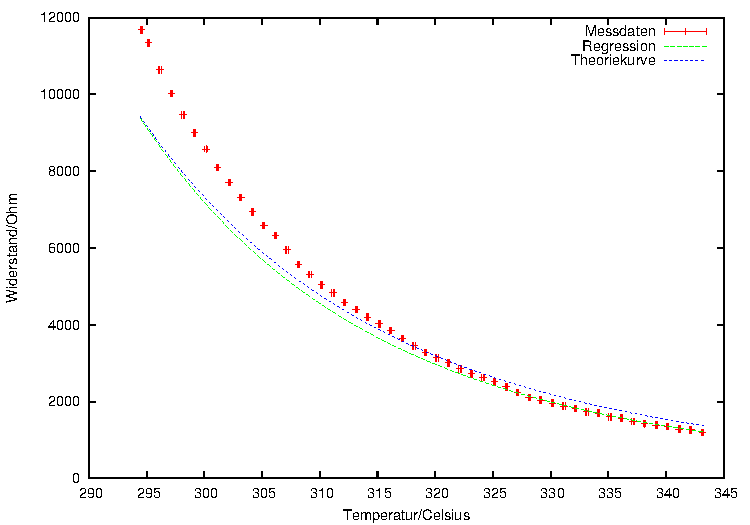
\includegraphics[ scale = 1.5]{1.pdf}
  	\caption[Graphische Auswertung Messdaten zur Eichung des NTC]{Graphische Auswertung Messdaten zur Eichung des NTC}
  \label{fig:1}
\end{figure}

\subsection{Diskussion}
%(immer) die gemessenen werte und die bestimmten werte über die messfehler mit literaturwerten oder untereinander vergleichen
%in welchem fehlerintervall des messwertes liegt der literaturwert oder der vergleichswert?
%wie ist der relative anteil des fehlers am messwert und damit die qualität unserer messung?
%in einem satz erklären, wie gut unser fehler und damit unsere messung ist
%kurz erläutern, wie systematische fehler unsere messung beeinflusst haben könnten
%(wichtig) zum schluss ansprechen, in wie weit die ergebnisse mit der theoretischen vorhersage übereinstimmen
%--------------------------------------------------------------------------------------------
%falls tabellen mit den messwerten zu lang werden, kann die section mit den messwerten auch hinter der diskussion angefügt bzw. eine section mit dem anhang eingefügt werden.
%1-----------------------------------------------1

Für B wurde ein Wert von 3988$^\circ$K erwartet mit einem Fehler von $\pm$79,76$^\circ$K, der bestimmte Wert weicht um 251$^\circ$K ab. Dieser große Abweichung vom erwartetem Wert kommt durch das schnelle aufheizten wodurch sich die Wärme in Heizwiderstand nicht schnell genug ausbreiten konnte.





\section{Regelschaltungen}
In diesem Versuchsabschnitt werden verschiedene Regelschaltungen untersucht. Es werden Zweiwegregler, Zweiwegregler mit Hysterese, Proportionalregler und Proportionalregler mit Integrator Untersucht.

\subsection{Zweiwegregler}
%kurz das ziel dieses versuchsteiles ansprechen, damit keine zwei überschriften direkt übereinander stehen!
%bei schwierigeren versuchen kann auch der theoretische hintergrund erläutert werden. (mit formeln, herleitungen und erklärungen)

In diesem Versuchsteil wird die Temperaturregulierung mittels eines Zweiwegreglers untersucht. Dieser unterscheidet nur zwischen des Zuständen Temperatur ist größer als der Sollwert oder Temperatur ist kleiner als Sollwert und reagiert dem entsprechend. Der Vorteil eines Zweiwegreglers ist, dass er sehr einfach aufzubauen ist. Nachteilig ist jedoch sein schlechtes Regelverhalten.

\subsubsection*{Verwendete Geräte}
%(immer) eine skizze oder ein foto einfügen, die geräte/materialien !nummerieren! und z.b. eine legende dazu schreiben, besser wäre es das ganze in einem Fließtext gut zu beschreiben.
%falls am anfang des versuches nicht klar ist, was alles verwendet wird, wenn möglich erst am ende ein großes foto von den verwendeten materialien machen!\\

Es werden ein Netzgerät, Widerstände, Kondensatoren, ein Oszilloskop, ein Op-Amp, ein Transistor, ein Lüfter und eine LED verwendet.


\subsubsection*{Versuchsaufbau}
%skizze zum versuchsaufbau (oder foto) einfügen,   es muss erklärt werden wie das ganze funktioniert und welche speziellen einstellungen verwendet wurden (z.b. welche knöpfe an den geräten für die messung verdreht wurden)

Die Werte der jeweiligen Bauteile sind im Schaltplan angegeben. 

\begin{figure}[H] 
  \centering
    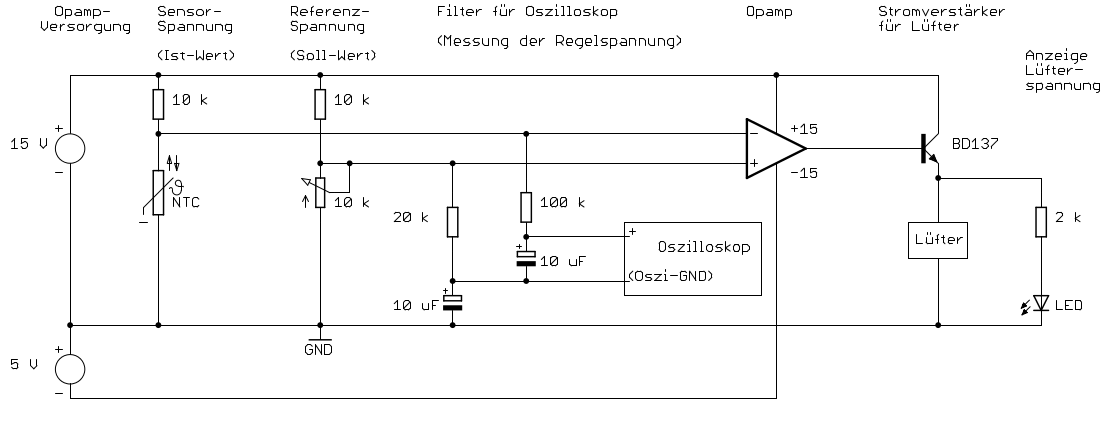
\includegraphics[ scale = 0.45]{Auf_2_1_1.png}
  	\caption[Schaltskizze des Zweiwegreglers]{Schaltskizze des Zweiwegreglers\footnotemark}
  \label{fig:auf_2_1_1}
\end{figure}
\footnotetext{Abbildungsteile entnommen von http://www.atlas.uni-wuppertal.de/$\sim$kind/ep7\_14.pdf am 06.12.2014}

Der Aufbau lässt sich auch vereinfacht darstellen (Abbildung \ref{fig:auf_2_1_2}). Im fort folgendem werden nur die vereinfachten Schaltskizzen angegeben.

\begin{figure}[H] 
  \centering
    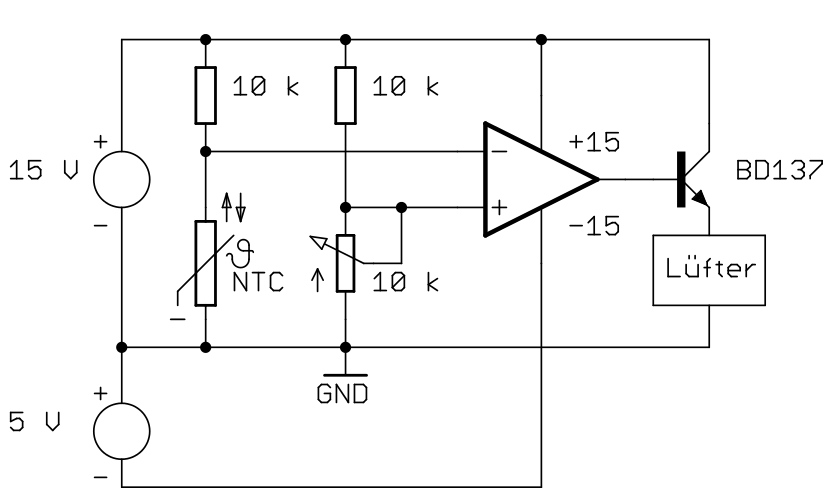
\includegraphics[ scale = 0.45]{Auf_2_1_2.png}
  	\caption[Vereinfachte Schaltskizze des Zweiwegreglers]{Vereinfachte Schaltskizze des Zweiwegreglers\footnotemark}
  \label{fig:auf_2_1_2}
\end{figure}
\footnotetext{Abbildungsteile entnommen von http://www.atlas.uni-wuppertal.de/$\sim$kind/ep7\_14.pdf am 06.12.2014}


\subsubsection*{Versuchsdurchführung}
%erklären, !was! wir machen, !warum! wir das machen und mit welchem ziel
%(wichtig) präzize erklären, wie bei dem versuch vorgegangen und was gemacht wurde

Es wir die Schaltung nach Abbildung \ref{fig:auf_2_1_1} aufgebaut. Dann wird das Netzgerät eingeschaltet und der Hitzewiderstand solange erwärmt, bis eine Temperatur von 50$^\circ$C auf dem Digitalthermometer angezeigt wird, die Solltemperatur wird mit dem 10k$\Omega$ Potentiometer so eingestellt. Wenn das Digitalthermometer 50$^\circ$C anzeigt wird die Spannung zwischen dem Invertierendem Eingang und der Masse gemessen. Dann soll der Temperaturverlauf in Abhängigkeit der Zeit gemessen werden, dafür wird die Heizspannung auf den Maximalwert aufgedreht und das Netzgerät eingeschaltet. Die Zeit wurde dabei mit von einer Person angesagt und die andere hat dann die Temperatur abgelesen. Die Messung beginnt ab dem Einschalten des Netzgerätes. Zum Schluss soll der die Eingangsspannung des Op-Amp untersucht werden. Dafür wird das Netzgerät eingeschaltet und und das Verhalten mit dem Oszilloskop aufgenommen.

\subsubsection*{Messergebnisse}
%die messwerte in !übersichtlichen! tabellen angegeben
%zu viele kleine tabellen in große tabellen überführen!
%zu große tabellen mit dem [scale]-befehl scalieren oder (falls zu lang) in zwei kleinere tabellen aufteilen
%(wichtig) vor !jeder! tabelle sagen, was gemessen wurde und wie die fehler gewählt wurden und ausreichend !erklären!, !warum! wir unsere fehler grade so gewählt haben

Der Fehler der Zeit wurde mit 0,5s angenommen, da eine Person sagen musste wann der Wert aufgenommen werden sollte und die andere Person dann die Temperatur ablesen musste. Der Fehler der Temperatur wurde mit der Ableseungenauigkeit bestimmt und beträgt 0,1C.

\begin{table}[htbp]
\begin{center}
\begin{tabular}{|r|r|}
\hline
t/s & T/$^\circ$C \\ \hline
0 & 50,7 \\ \hline
5 & 50,6 \\ \hline
10 & 50 \\ \hline
15 & 49,5 \\ \hline
20 & 49,2 \\ \hline
25 & 48,9 \\ \hline
30 & 48,7 \\ \hline
35 & 48,7 \\ \hline
40 & 48,5 \\ \hline
45 & 48,6 \\ \hline
50 & 48,5 \\ \hline
55 & 48,4 \\ \hline
60 & 48,4 \\ \hline
65 & 48,4 \\ \hline
70 & 48,4 \\ \hline
75 & 48,3 \\ \hline
80 & 48,4 \\ \hline
85 & 48,3 \\ \hline
\end{tabular}
\end{center}
\caption{Messdaten der Temperatur in Abhängigkeit der Zeit für den Zweiwegregler}
\label{tab:2_1}
\end{table}


\subsubsection*{Auswertung}
%zuerst !alle! errechneten werte entweder in ganzen sätzen aufzählen, oder in tabellen (übersichtlicher) dargestellen, sowie auf die verwendeten formeln verweisen (die referenzierung der formel kann in der überschrift stehen)
%kurz erwähnen (vor der tabelle), warum wir das ganze ausrechnen bzw. was wir dort ausrechnen
%danach histogramme und plots erstellen, wobei wenn möglich funktionen durch die plots gelegt werden (zur not können auch splines benutzt werden, was aber angegeben werden muss)
%bei fits immer die funktion und das reduzierte chiquadrat mit angegeben, wobei auf verständlichkeit beim entziffern der zehnerpotenzen geachtet werden muss z.b. f(x)=(wert+-fehler)\cdot10^{irgendeine zahl}\cdot x + (wert+-fehler)\cdot10^{irgendeine zahl}
%bei jedem fit erklären, nach welchem zusammenhang gefittet wurde und warum!
%bei plots darauf achten, dass die achsenbeschriftung (auch die tics) die richtige größe haben und die legende im plot nicht die messwerte verdeckt
%kurz die aufgabenstellung abhandeln
%2-----------------------------------------------2

Im ersten Teil soll die Temperatur auf 50$^\circ$C geregelt werden und die Spannung am invertiertem Eingang gemessen werden. Theoretisch ergibt sich die erwartete Spannung aus Gleichung \ref{eqn:ntc}, ausgewertet bei 50$^\circ$C und bestimmten der Spannung über den Spannungsteiler NTC. Es ergibt sich ein Wert von 3,93V. Gemessen wurde ein Wert von 3,88$\pm$0,06V.

Im zweitem Teil sollte die Regelkurve aufgenommen werden. Der Plot der Messdaten ist in Abbildung \ref{fig:2_1} zu sehen.

\begin{figure}[H] 
  \centering
    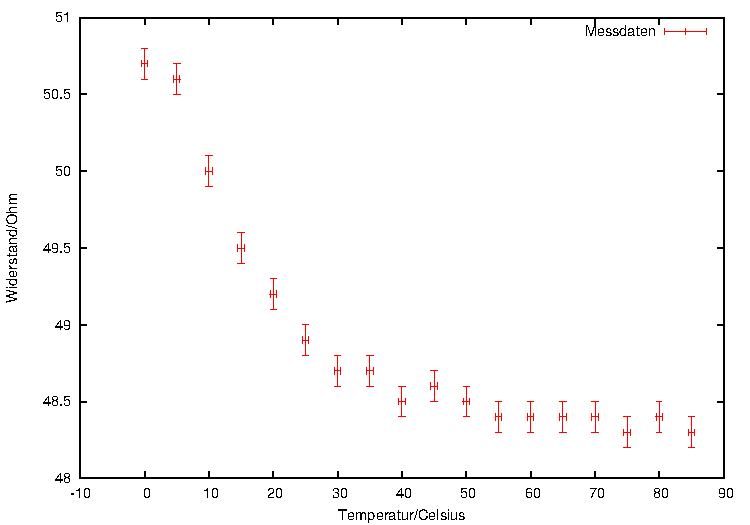
\includegraphics[ scale = 1]{2_1_1.pdf}
  	\caption[Graphische Auswertung der Regelkurve für den Zweiwegregler]{Graphische Auswertung der Regelkurve für den Zweiwegregler}
  \label{fig:2_1}
\end{figure}

Im dritten Versuchsteil soll das Verhalten der Eingangsspannung untersucht werden. Dafür wurde die Eingangsspannung mit dem Oszilloskop aufgenommen, der Verlauf ist in Abbildung \ref{fig:2_1_2} zu sehen.

\begin{figure}[H] 
  \centering
    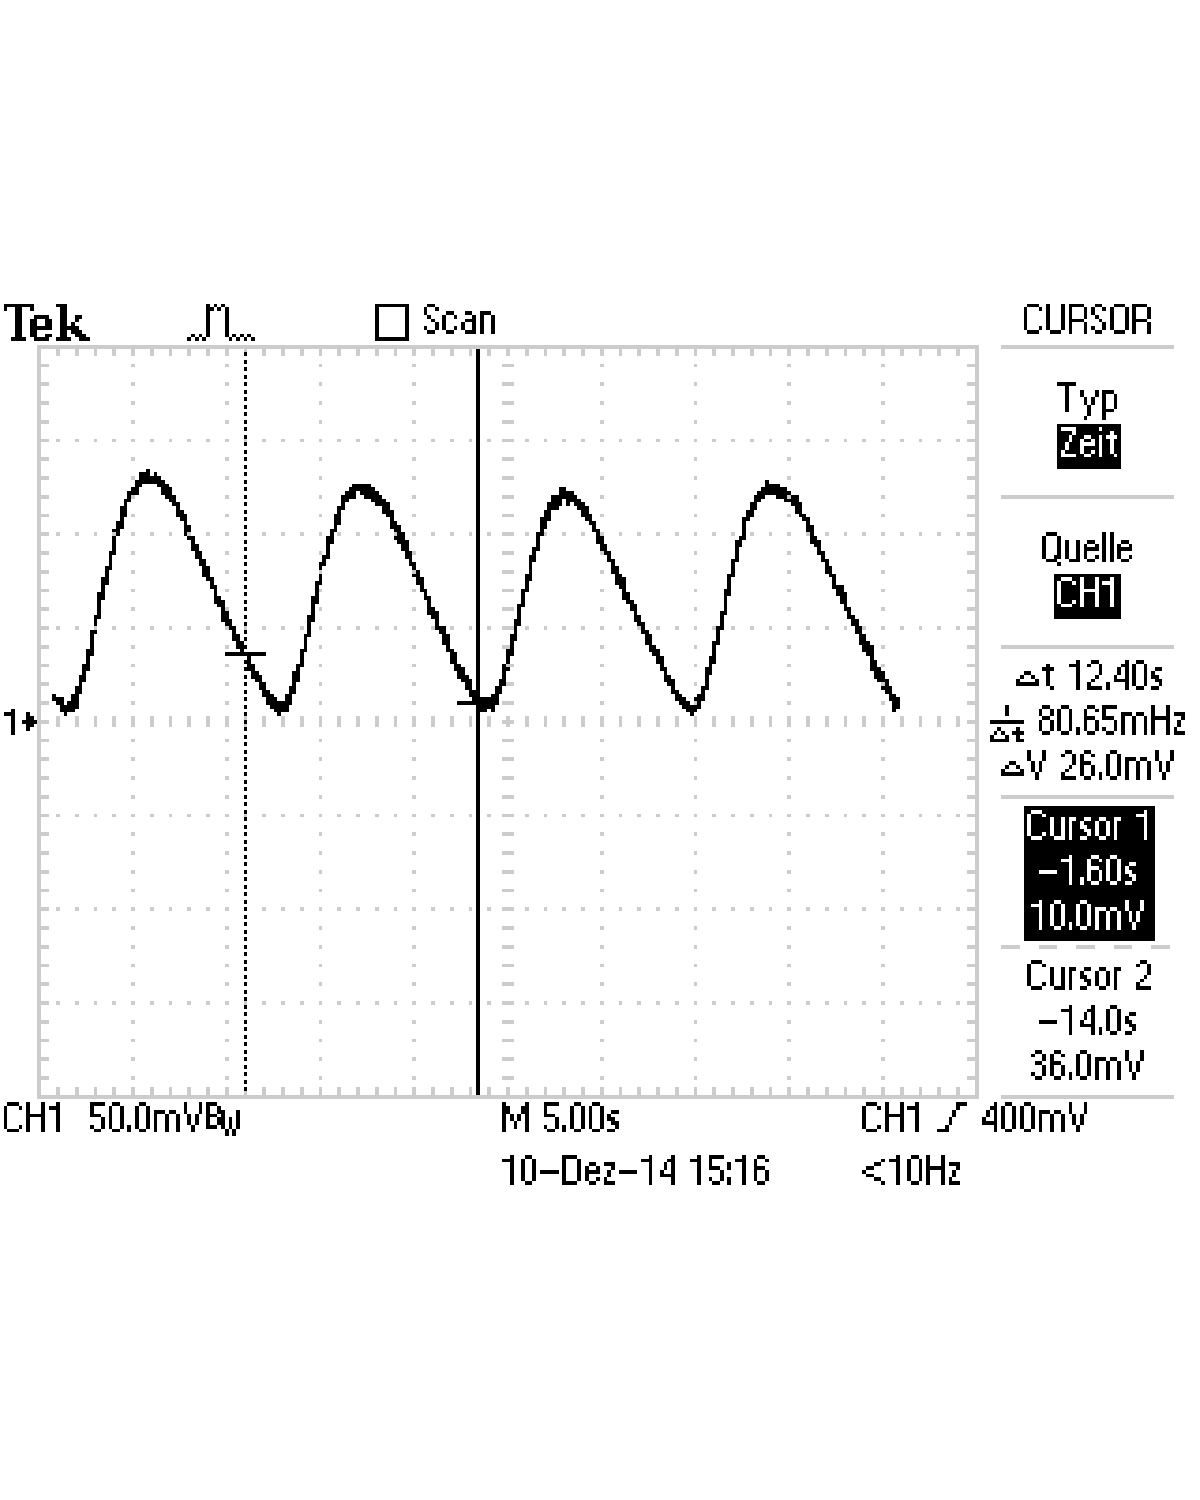
\includegraphics[ scale = 0.6]{2_1_2.pdf}
  	\caption[Eingasspannung]{Eingasspannung}
  \label{fig:2_1}
\end{figure}

\subsubsection*{Diskussion}
%(immer) die gemessenen werte und die bestimmten werte über die messfehler mit literaturwerten oder untereinander vergleichen
%in welchem fehlerintervall des messwertes liegt der literaturwert oder der vergleichswert?
%wie ist der relative anteil des fehlers am messwert und damit die qualität unserer messung?
%in einem satz erklären, wie gut unser fehler und damit unsere messung ist
%kurz erläutern, wie systematische fehler unsere messung beeinflusst haben könnten
%(wichtig) zum schluss ansprechen, in wie weit die ergebnisse mit der theoretischen vorhersage übereinstimmen
%--------------------------------------------------------------------------------------------
%falls tabellen mit den messwerten zu lang werden, kann die section mit den messwerten auch hinter der diskussion angefügt bzw. eine section mit dem anhang eingefügt werden.
%1-----------------------------------------------1
Die Spannung am invertiertem Eingang bei 50$^\circ$C wurde mit 3,88$\pm$0,06V gemessen, erwartet wurde eine Wert von 3,93V. Der erwartete Wert liegt innerhalb des ersten Fehlerintervalls des gemessenen Wertes. Die Regelkurve zeigt, wie sich die Temperatur der Solltemperatur annähert und dann schwach um den Sollwert schwingt. Das Verhalten der Eingangsspannung verhält sich wie erwartet, sobald die Solltemperatur überschritten wird steigt die Eingasspannung und wenn die Solltemperatur unterschritten wird, fällt die Spannung ab.



\subsection{Zweiwegregler mit Hysterese}
%kurz das ziel dieses versuchsteiles ansprechen, damit keine zwei überschriften direkt übereinander stehen!
%bei schwierigeren versuchen kann auch der theoretische hintergrund erläutert werden. (mit formeln, herleitungen und erklärungen)

In diesem Versuchsteil wird die Reglung der Temperatur über eine Zweiwegreglung mit Hysterese untersucht. Der Vorteil dieser Schaltung ist, dass durch die Hysterese die Regelung erst etwas später eintritt.

\subsubsection*{Verwendete Geräte}
%(immer) eine skizze oder ein foto einfügen, die geräte/materialien !nummerieren! und z.b. eine legende dazu schreiben, besser wäre es das ganze in einem Fließtext gut zu beschreiben.
%falls am anfang des versuches nicht klar ist, was alles verwendet wird, wenn möglich erst am ende ein großes foto von den verwendeten materialien machen!\\

Es werden ein Netzgerät, Widerstände, Kondensatoren, ein Oszilloskop, ein Op-Amp, ein Transistor und ein Lüfter verwendet.

\subsubsection*{Versuchsaufbau}
%skizze zum versuchsaufbau (oder foto) einfügen,   es muss erklärt werden wie das ganze funktioniert und welche speziellen einstellungen verwendet wurden (z.b. welche knöpfe an den geräten für die messung verdreht wurden)

Die Hysterese wird dadurch erreicht, dass Eingang und Ausgang mit einem Widerstand verbunden werden. Hier ist Rh der Widerstand und er hat eine Wert von 20k$\Omega$ bis 100k$\Omega$.

\begin{figure}[H] 
  \centering
    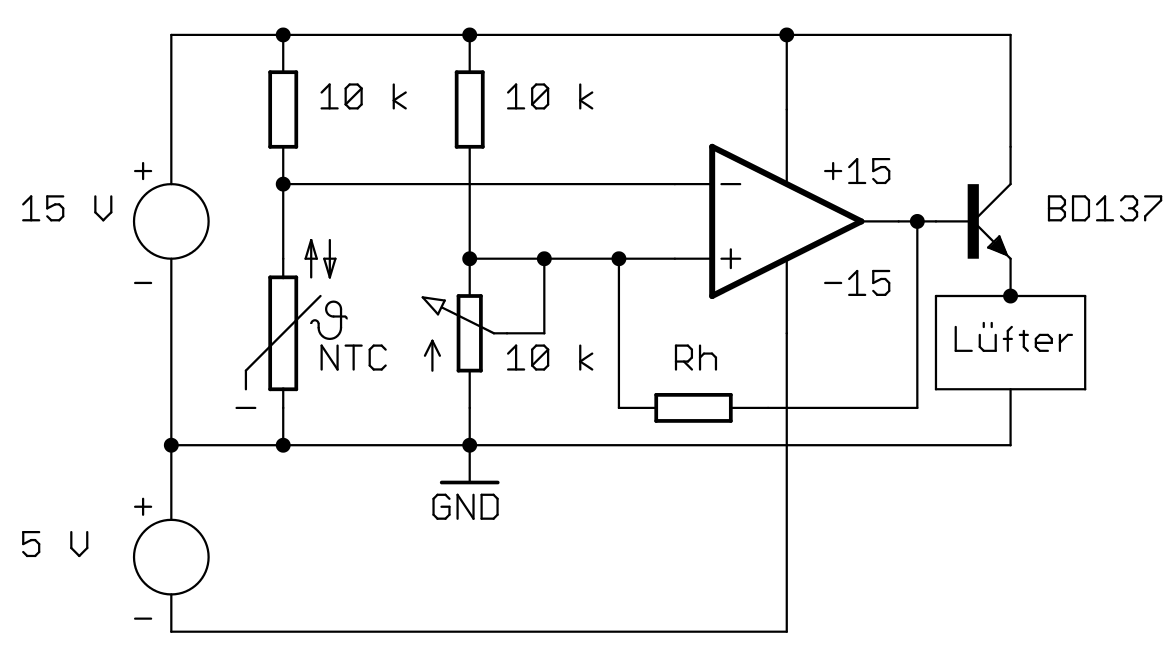
\includegraphics[ scale = 0.45]{Auf_2_2.png}
  	\caption[Vereinfachte Schaltskizze des Zweiwegreglers mit Hysterese]{Vereinfachte Schaltskizze des Zweiwegreglers  mit Hysterese\footnotemark}
  \label{fig:auf_2_2}
\end{figure}
\footnotetext{Abbildungsteile entnommen von http://www.atlas.uni-wuppertal.de/$\sim$kind/ep7\_14.pdf am 06.12.2014}

\subsubsection*{Versuchsdurchführung}
%erklären, !was! wir machen, !warum! wir das machen und mit welchem ziel
%(wichtig) präzize erklären, wie bei dem versuch vorgegangen und was gemacht wurde

Zu erst wurde die Schaltung nach Abbildung \ref{fig:auf_2_2} aufgebaut. Dann sollte die Eingangsspannung aufgenommen werden. Dafür wird das Netzgerät eingeschaltet und mit dem Oszilloskop die Eingangsspannung aufgenommen.


\subsubsection*{Auswertung}
%zuerst !alle! errechneten werte entweder in ganzen sätzen aufzählen, oder in tabellen (übersichtlicher) dargestellen, sowie auf die verwendeten formeln verweisen (die referenzierung der formel kann in der überschrift stehen)
%kurz erwähnen (vor der tabelle), warum wir das ganze ausrechnen bzw. was wir dort ausrechnen
%danach histogramme und plots erstellen, wobei wenn möglich funktionen durch die plots gelegt werden (zur not können auch splines benutzt werden, was aber angegeben werden muss)
%bei fits immer die funktion und das reduzierte chiquadrat mit angegeben, wobei auf verständlichkeit beim entziffern der zehnerpotenzen geachtet werden muss z.b. f(x)=(wert+-fehler)\cdot10^{irgendeine zahl}\cdot x + (wert+-fehler)\cdot10^{irgendeine zahl}
%bei jedem fit erklären, nach welchem zusammenhang gefittet wurde und warum!
%bei plots darauf achten, dass die achsenbeschriftung (auch die tics) die richtige größe haben und die legende im plot nicht die messwerte verdeckt
%kurz die aufgabenstellung abhandeln
%2-----------------------------------------------2

Die veränderten Umschaltpunkt kommen dadurch zustande, dass durch die Rückkopplung auch nach erreichen des Sollwertes noch ein Eingangssignal vorhanden ist. Das Verhalten der Eingangsspannung ist in Abbildung \ref{fig:2_2} zu sehen. Die Hysterese ist deutlich an den Stellen mit der starke Steigung bzw. mit dem starken Abfall zu sehen.

\begin{figure}[H] 
  \centering
    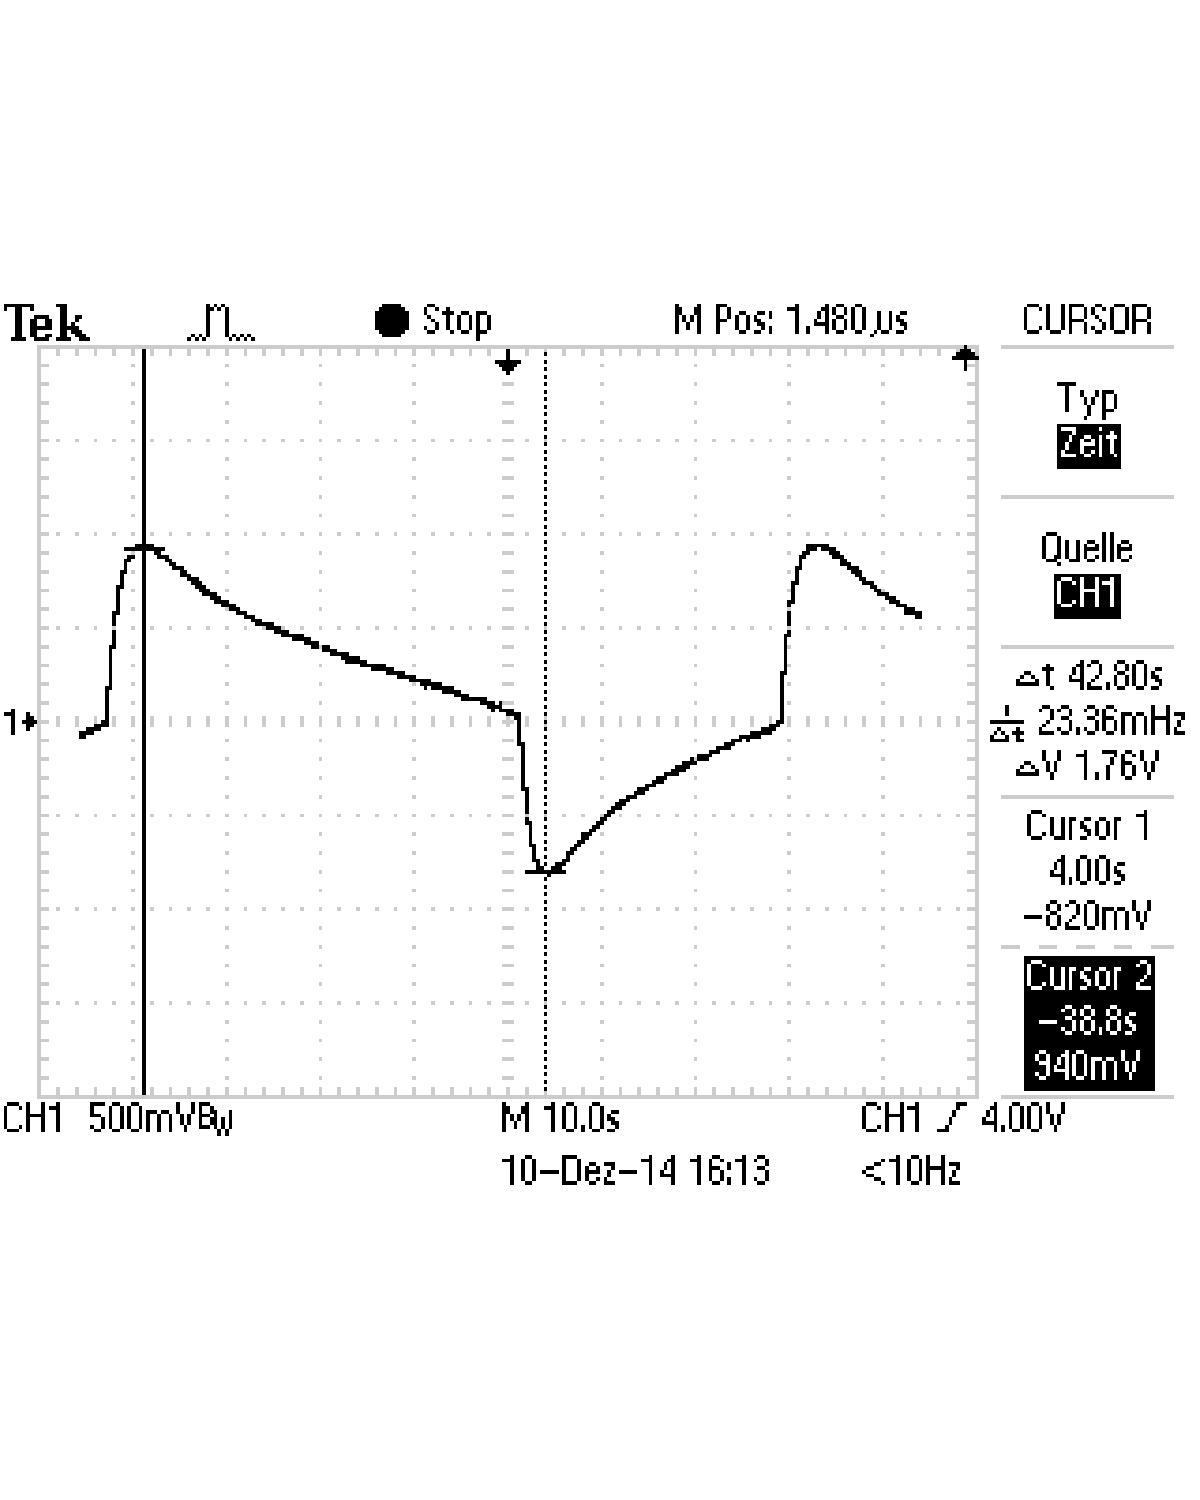
\includegraphics[ scale = 0.6]{2_2.pdf}
  	\caption[Graphische Auswertung der Regelkurve für den Zweiwegregler]{Graphische Auswertung der Regelkurve für den Zweiwegregler}
  \label{fig:2_2}
\end{figure}

\subsubsection*{Diskussion}
%(immer) die gemessenen werte und die bestimmten werte über die messfehler mit literaturwerten oder untereinander vergleichen
%in welchem fehlerintervall des messwertes liegt der literaturwert oder der vergleichswert?
%wie ist der relative anteil des fehlers am messwert und damit die qualität unserer messung?
%in einem satz erklären, wie gut unser fehler und damit unsere messung ist
%kurz erläutern, wie systematische fehler unsere messung beeinflusst haben könnten
%(wichtig) zum schluss ansprechen, in wie weit die ergebnisse mit der theoretischen vorhersage übereinstimmen
%--------------------------------------------------------------------------------------------
%falls tabellen mit den messwerten zu lang werden, kann die section mit den messwerten auch hinter der diskussion angefügt bzw. eine section mit dem anhang eingefügt werden.
%1-----------------------------------------------1

Wie erwartet ergab sich durch die Hysterese ein verspäteter Einschalts- und Ausschaltszeitpunkt. Dies ist deutlich in Abbildung \ref{fig:2_2} zu sehen.

\subsection{Proportionalregler}
%kurz das ziel dieses versuchsteiles ansprechen, damit keine zwei überschriften direkt übereinander stehen!
%bei schwierigeren versuchen kann auch der theoretische hintergrund erläutert werden. (mit formeln, herleitungen und erklärungen)

In diesem Versuchsteil wird der Proportionalregler untersucht, er ermöglicht eine kontinuierliche Regulierung der Drehzahl des Lüfters.

\subsubsection*{Verwendete Geräte}
%(immer) eine skizze oder ein foto einfügen, die geräte/materialien !nummerieren! und z.b. eine legende dazu schreiben, besser wäre es das ganze in einem Fließtext gut zu beschreiben.
%falls am anfang des versuches nicht klar ist, was alles verwendet wird, wenn möglich erst am ende ein großes foto von den verwendeten materialien machen!\\

Es werden ein Netzgerät, Widerstände, Kondensatoren, ein Oszilloskop, ein Op-Amp, ein Transistor und ein Lüfter verwendet.


\subsubsection*{Versuchsaufbau}
%skizze zum versuchsaufbau (oder foto) einfügen,   es muss erklärt werden wie das ganze funktioniert und welche speziellen einstellungen verwendet wurden (z.b. welche knöpfe an den geräten für die messung verdreht wurden)

Um den Proportionalregler zu realisierten, wird der invertierende Eingang über einen Widerstand mit dem Ausgang rückgekoppelt. In dem Aufbau in Abbildung \ref{fig:auf_2_3} wird der Widerstand Rf für die Rückkopplung verwendet, es handelt sich um einen 1M$\Omega$. Ri ist ein 4,7k$\Omega$ Widerstand.

\begin{figure}[H] 
  \centering
    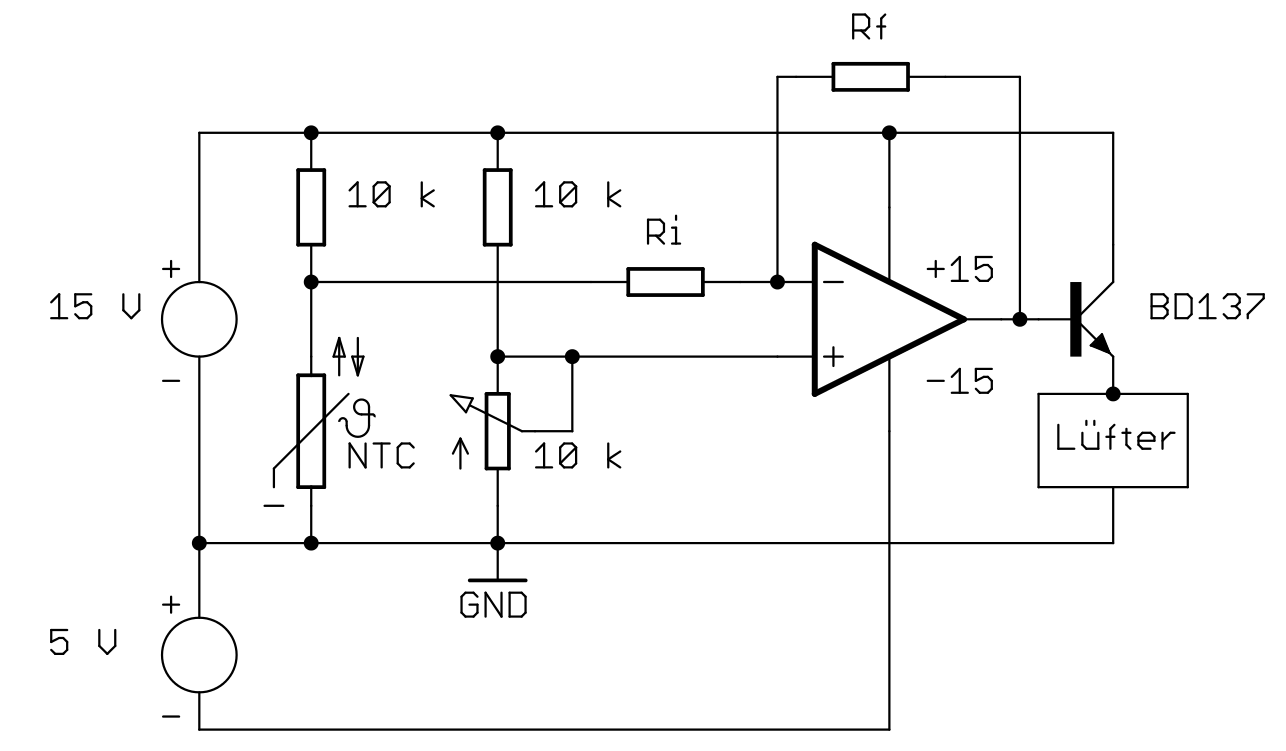
\includegraphics[ scale = 0.4]{Auf_2_3.png}
  	\caption[Vereinfachte Schaltskizze des Proportionalreglers]{Vereinfachte Schaltskizze des Proportionalreglers\footnotemark}
  \label{fig:auf_2_3}
\end{figure}
\footnotetext{Abbildungsteile entnommen von http://www.atlas.uni-wuppertal.de/$\sim$kind/ep7\_14.pdf am 06.12.2014}


\subsubsection*{Versuchsdurchführung}
%erklären, !was! wir machen, !warum! wir das machen und mit welchem ziel
%(wichtig) präzize erklären, wie bei dem versuch vorgegangen und was gemacht wurde
\subsubsection*{Messergebnisse}
%die messwerte in !übersichtlichen! tabellen angegeben
%zu viele kleine tabellen in große tabellen überführen!
%zu große tabellen mit dem [scale]-befehl scalieren oder (falls zu lang) in zwei kleinere tabellen aufteilen
%(wichtig) vor !jeder! tabelle sagen, was gemessen wurde und wie die fehler gewählt wurden und ausreichend !erklären!, !warum! wir unsere fehler grade so gewählt haben
\subsubsection*{Auswertung}
%zuerst !alle! errechneten werte entweder in ganzen sätzen aufzählen, oder in tabellen (übersichtlicher) dargestellen, sowie auf die verwendeten formeln verweisen (die referenzierung der formel kann in der überschrift stehen)
%kurz erwähnen (vor der tabelle), warum wir das ganze ausrechnen bzw. was wir dort ausrechnen
%danach histogramme und plots erstellen, wobei wenn möglich funktionen durch die plots gelegt werden (zur not können auch splines benutzt werden, was aber angegeben werden muss)
%bei fits immer die funktion und das reduzierte chiquadrat mit angegeben, wobei auf verständlichkeit beim entziffern der zehnerpotenzen geachtet werden muss z.b. f(x)=(wert+-fehler)\cdot10^{irgendeine zahl}\cdot x + (wert+-fehler)\cdot10^{irgendeine zahl}
%bei jedem fit erklären, nach welchem zusammenhang gefittet wurde und warum!
%bei plots darauf achten, dass die achsenbeschriftung (auch die tics) die richtige größe haben und die legende im plot nicht die messwerte verdeckt
%kurz die aufgabenstellung abhandeln
%2-----------------------------------------------2
\subsubsection*{Diskussion}
%(immer) die gemessenen werte und die bestimmten werte über die messfehler mit literaturwerten oder untereinander vergleichen
%in welchem fehlerintervall des messwertes liegt der literaturwert oder der vergleichswert?
%wie ist der relative anteil des fehlers am messwert und damit die qualität unserer messung?
%in einem satz erklären, wie gut unser fehler und damit unsere messung ist
%kurz erläutern, wie systematische fehler unsere messung beeinflusst haben könnten
%(wichtig) zum schluss ansprechen, in wie weit die ergebnisse mit der theoretischen vorhersage übereinstimmen
%--------------------------------------------------------------------------------------------
%falls tabellen mit den messwerten zu lang werden, kann die section mit den messwerten auch hinter der diskussion angefügt bzw. eine section mit dem anhang eingefügt werden.
%1-----------------------------------------------1



\subsection{Proportionalregler mit Integrator}
%kurz das ziel dieses versuchsteiles ansprechen, damit keine zwei überschriften direkt übereinander stehen!
%bei schwierigeren versuchen kann auch der theoretische hintergrund erläutert werden. (mit formeln, herleitungen und erklärungen)

In diesem Versuchsaufbau wird ein Proportionalregler mit Integrator untersucht. Durch den Integrator können Schwingungen der Regelung ausgeglichen werden, zudem ist die Regelwirkung bei einem Verzug der Wirkung stärker.

\subsubsection*{Verwendete Geräte}
%(immer) eine skizze oder ein foto einfügen, die geräte/materialien !nummerieren! und z.b. eine legende dazu schreiben, besser wäre es das ganze in einem Fließtext gut zu beschreiben.
%falls am anfang des versuches nicht klar ist, was alles verwendet wird, wenn möglich erst am ende ein großes foto von den verwendeten materialien machen!\\

Es werden ein Netzgerät, Widerstände, Kondensatoren, ein Oszilloskop, ein Op-Amp, ein Transistor und ein Lüfter verwendet.


\subsubsection*{Versuchsaufbau}
%skizze zum versuchsaufbau (oder foto) einfügen,   es muss erklärt werden wie das ganze funktioniert und welche speziellen einstellungen verwendet wurden (z.b. welche knöpfe an den geräten für die messung verdreht wurden)

Um dem Proportionalregler noch einen Integrator hinzuzufügen wird noch ein Kondensator in Reihe zu Rf geschaltet. C beträgt dabei 100$\mu$F, damit das Signal nicht wegläuft wird noch ein 100M$\Omega$ Widerstand parallel zu C geschaltet.

\begin{figure}[H] 
  \centering
    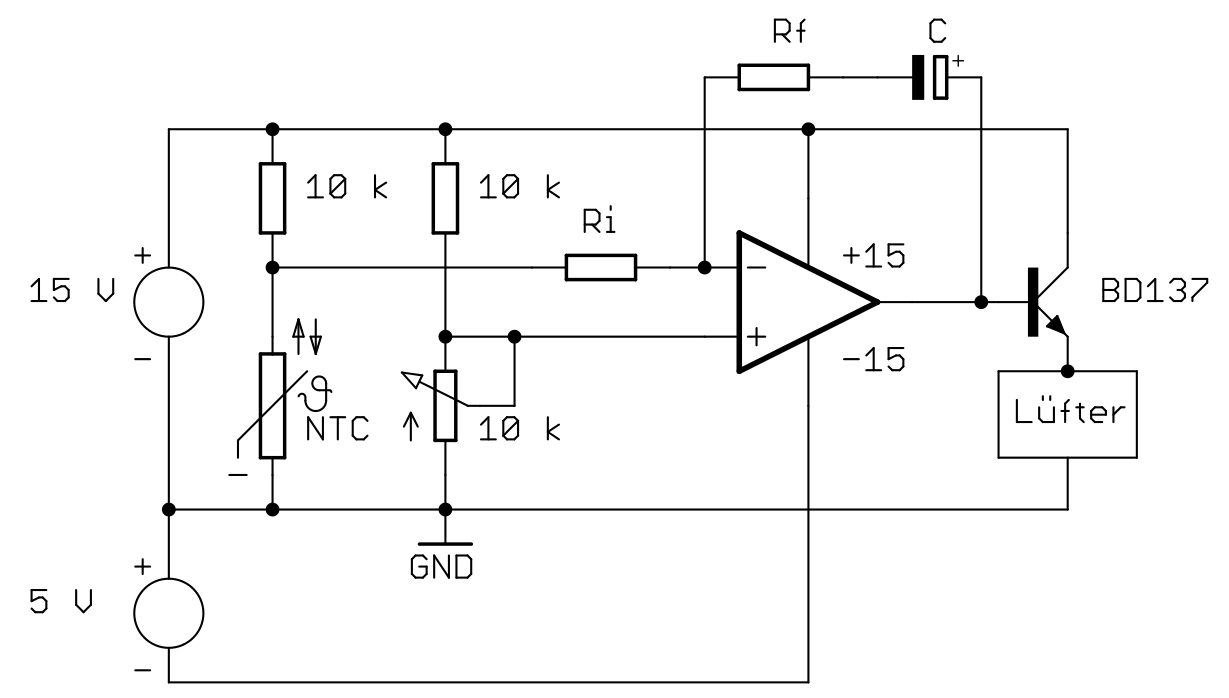
\includegraphics[ scale = 0.4]{Auf_2_4.png}
  	\caption[Vereinfachte Schaltskizze des Proportionalreglers mit Integrator]{Vereinfachte Schaltskizze des Proportionalreglers mit Integrator\footnotemark}
  \label{fig:auf_2_4}
\end{figure}
\footnotetext{Abbildungsteile entnommen von http://www.atlas.uni-wuppertal.de/$\sim$kind/ep7\_14.pdf am 06.12.2014}

\subsubsection*{Versuchsdurchführung}
%erklären, !was! wir machen, !warum! wir das machen und mit welchem ziel
%(wichtig) präzize erklären, wie bei dem versuch vorgegangen und was gemacht wurde
\subsubsection*{Messergebnisse}
%die messwerte in !übersichtlichen! tabellen angegeben
%zu viele kleine tabellen in große tabellen überführen!
%zu große tabellen mit dem [scale]-befehl scalieren oder (falls zu lang) in zwei kleinere tabellen aufteilen
%(wichtig) vor !jeder! tabelle sagen, was gemessen wurde und wie die fehler gewählt wurden und ausreichend !erklären!, !warum! wir unsere fehler grade so gewählt haben
\subsubsection*{Auswertung}
%zuerst !alle! errechneten werte entweder in ganzen sätzen aufzählen, oder in tabellen (übersichtlicher) dargestellen, sowie auf die verwendeten formeln verweisen (die referenzierung der formel kann in der überschrift stehen)
%kurz erwähnen (vor der tabelle), warum wir das ganze ausrechnen bzw. was wir dort ausrechnen
%danach histogramme und plots erstellen, wobei wenn möglich funktionen durch die plots gelegt werden (zur not können auch splines benutzt werden, was aber angegeben werden muss)
%bei fits immer die funktion und das reduzierte chiquadrat mit angegeben, wobei auf verständlichkeit beim entziffern der zehnerpotenzen geachtet werden muss z.b. f(x)=(wert+-fehler)\cdot10^{irgendeine zahl}\cdot x + (wert+-fehler)\cdot10^{irgendeine zahl}
%bei jedem fit erklären, nach welchem zusammenhang gefittet wurde und warum!
%bei plots darauf achten, dass die achsenbeschriftung (auch die tics) die richtige größe haben und die legende im plot nicht die messwerte verdeckt
%kurz die aufgabenstellung abhandeln
%2-----------------------------------------------2
\subsubsection*{Diskussion}
%(immer) die gemessenen werte und die bestimmten werte über die messfehler mit literaturwerten oder untereinander vergleichen
%in welchem fehlerintervall des messwertes liegt der literaturwert oder der vergleichswert?
%wie ist der relative anteil des fehlers am messwert und damit die qualität unserer messung?
%in einem satz erklären, wie gut unser fehler und damit unsere messung ist
%kurz erläutern, wie systematische fehler unsere messung beeinflusst haben könnten
%(wichtig) zum schluss ansprechen, in wie weit die ergebnisse mit der theoretischen vorhersage übereinstimmen
%--------------------------------------------------------------------------------------------
%falls tabellen mit den messwerten zu lang werden, kann die section mit den messwerten auch hinter der diskussion angefügt bzw. eine section mit dem anhang eingefügt werden.
%1-----------------------------------------------1

\section{Fazit}
%im fazit nochmal alles zusammenfassen und den verlauf der messung abschätzen
%gravierende sytematische probleme bei den messungen nochmal betonen und die wertigkeit unserer ergebnisse einordnen
\end{document}

